\section{TRATAMENTOS AOS DADOS}
\label{sec:tratamentosDados}

Nesta seção são apresentados resumidamente os tratamentos e pré-processamentos realizados sobre os dados da distribuição espaço-temporal dos casos de Influenza no ano de 2009 na cidade de Cascavel/PR, à obtenção de arquivos de entrada utilizados em simulações computacionais. Especificamente, os casos de Influenza são utilizados à obtenção dos arquivos de sazonalidade e distribuição de agentes infectados durante a simulação. As informações obtidas do arquivo de sazonalidade são utilizadas durante a operação de contato entre agentes suscetíveis e infectantes ao controle da taxa de infecção, de acordo com os casos reais observados. O arquivo de distribuição é utilizado à inserção de agentes infectados no ambiente durante a execução de simulações, sendo esses agentes responsáveis pelo início do processo infeccioso da doença. As posições nas quais estes agentes são inseridos correspondem às posições de casos reais de Influenza que foram georreferenciados. 

O percentual de infecção dos agentes suscetíveis em contato com infectados é calculado utilizando-se três distintos parâmetros: os percentuais de infecção adotados às faixas etárias, o percentual de sazonalidade do ciclo em que ocorre o contato e uma constante de sazonalidade. Todos esses percentuais são definidos em arquivos de configuração da simulação que são gerados ou manualmente ou por meio do \textit{software} SIMULA. Os percentuais de infecção por faixa etária e a constante de sazonalidade foram definidos de forma empírica por meio de execução de testes. Os percentuais de sazonalidade por ciclo foram definidos com base na distribuição temporal dos casos de Influenza durante o ano de 2009. A Figura \ref{fig:percentuais_sazonalidade} ilustra o gráfico gerado a partir dos percentuais de sazonalidade.

\begin{figure}[H]
  \centering
  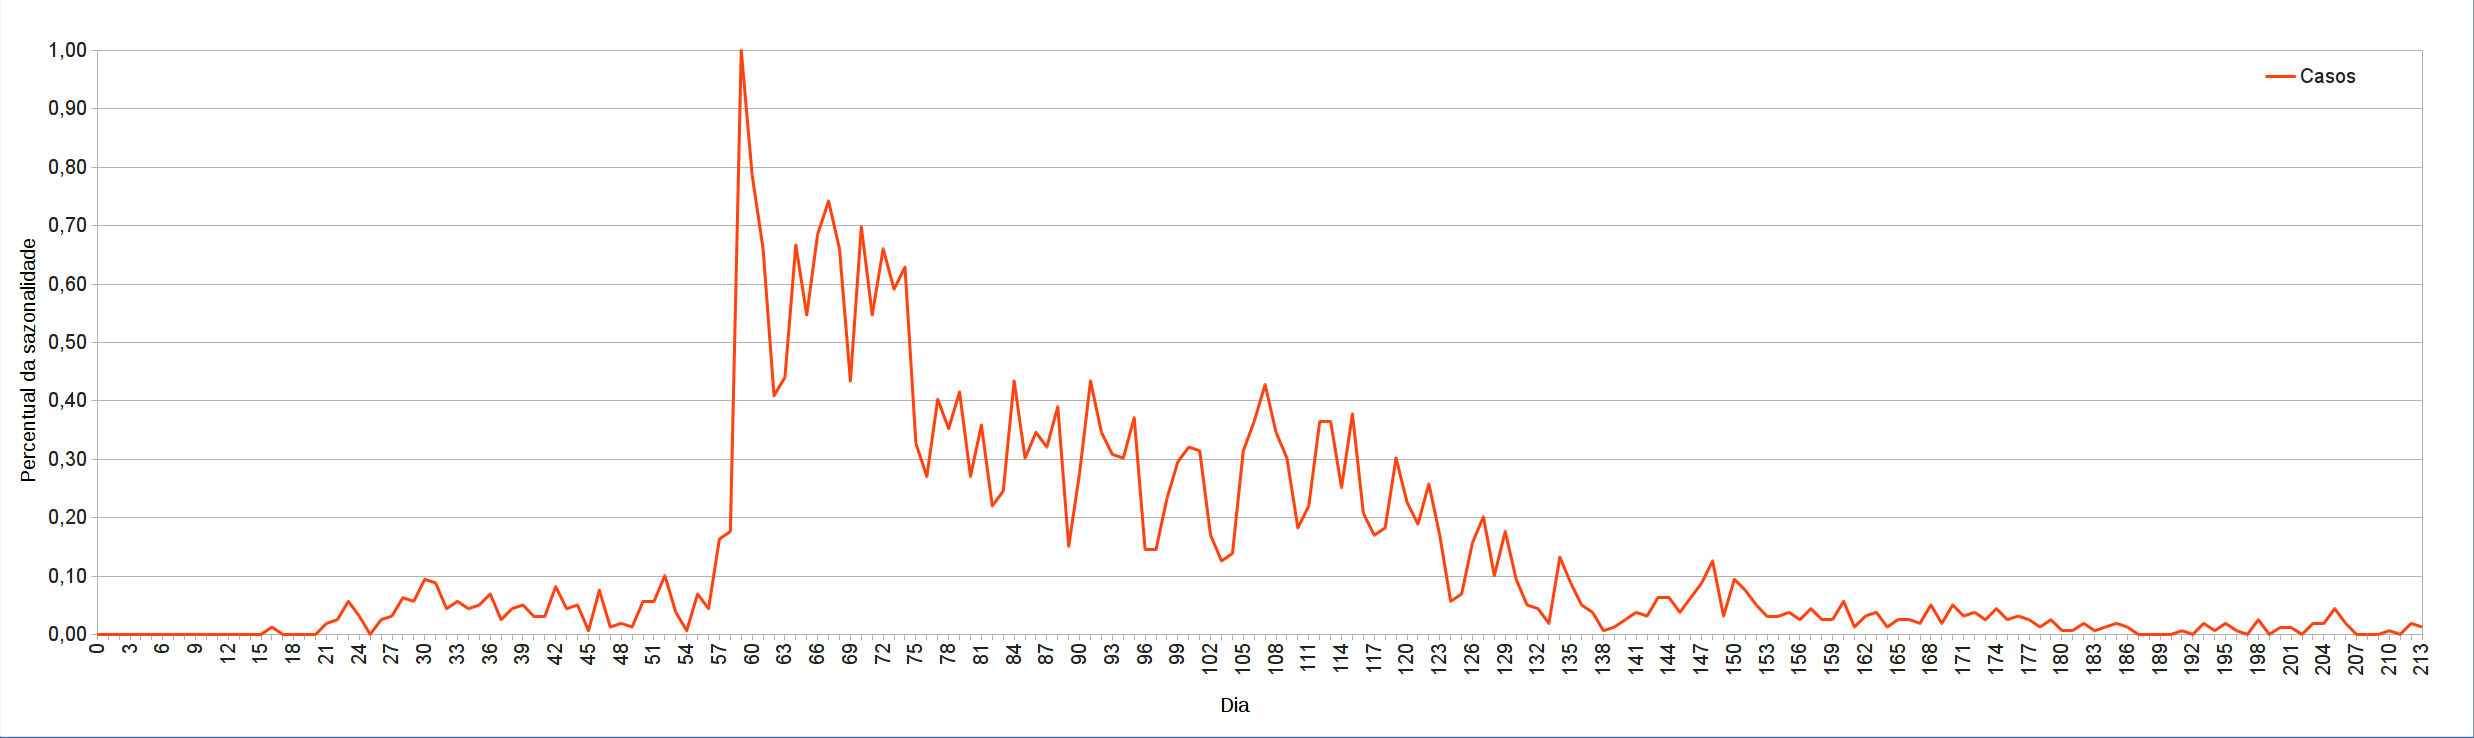
\includegraphics[width=1\textwidth]{Figuras/TratamentosDados/Sazonalidade.png}
  \caption{Distribuição temporal dos percentuais de sazonalidade}
  \label{fig:percentuais_sazonalidade}
\end{figure} 

À obtenção dos percentuais de sazonalidade por ciclo foram realizadas diversas atividades de pré-processamento sobre os dados originais que totalizavam $5.089$ casos de Influenza. Inicialmente foram removidos os casos não georreferenciados ou localizados em regiões não-urbanas da cidade de Cascavel/PR, como zonas rurais e distritos. Em sequência foram mantidos somente os casos com datas de ocorrência entre 17 de Junho e 31 de Dezembro de 2009, pois considerou-se estes casos mais significativos à propósitos de simulação. Após estas operações restaram $4.658$ casos. Estes casos foram então agrupados por dia de ocorrência dos primeiros sintomas e as quantidades foram normalizadas dentro do intervalo $[0.0, 1.0]$, que correspondem aos percentuais de sazonalidade empregados na simulação.

O arquivo de distribuição de agentes infectados ao longo da simulação é gerado pela função \textit{criarDistribuicaoAgentes}, que é ilustrada no Código \ref{cod:criarDistribuicaoAgentes}, Algoritmo \ref{alg:criarDistribuicaoAgentes} e Figura \ref{fig:criarDistribuicaoAgentes}. Na função são definidos manualmente percentuais de casos utilizados e frações de machos e fêmeas para cada faixa etária. Foram utilizadas as faixas etárias definidas pelo IBGE, que classificam os indivíduos com idade entre 0 e 14 anos como crianças, com idade entre 15 e 24 como jovens, com idade entre 25 e 29 anos como adultos e com idade maior que 59 como idosos. Atualmente, $3\%$ da quantidade total de casos são inseridos durante a execução da simulação. Para as crianças, $51\%$ são masculinos e $49\%$ são femininos. Para os jovens, $50\%$ são masculinos e $50\%$ são femininos. Para os adultos, $48\%$ são masculinos e $52\%$ são femininos. Por fim, para os idosos, $45\%$ são masculinos e $55\%$ são femininos. Na escolha dos casos que serão utilizados inicialmente o conjunto de todos os casos é agrupado por dia de ocorrência. Em seguida, para cada dia são mantidos $3\%$ dos casos. Os casos são então agrupados por faixa etária e os percentuais apresentados anteriormente são utilizados à atribuição aleatória dos sexos. O passo final do algoritmo consiste em atribuir uma posição para a inserção do agente no ambiente, já que os pontos originais dos casos georreferenciados podem não estar presentes no conjunto de pontos interpolados no ambiente. Neste caso, o ponto do ambiente que é mais próximo aquele do caso original é escolhido, considerando-se a distância euclidiana entre eles. 

\newpage